\textbf{Целью четвертой лабораторной работы} является знакомство с возможностями программы Microsoft Project по контролю за ходом реализации проекта.

\section*{Содержание проекта}

Команда разработчиков из 16 человек занимается созданием карты города на основе собственного модуля отображения. Проект должен быть завершен в течение шести месяцев. Бюджет проекта: 50 000 рублей.

\section*{Сведения о параметрах базового плана проекта}

Базовые даты начала и окончания проекта --- 1.03.2023 и 27.07.2023. Состояние проекта показано на рисунке \ref{img:start-project}.

\begin{figure}[H]
	\begin{center}
		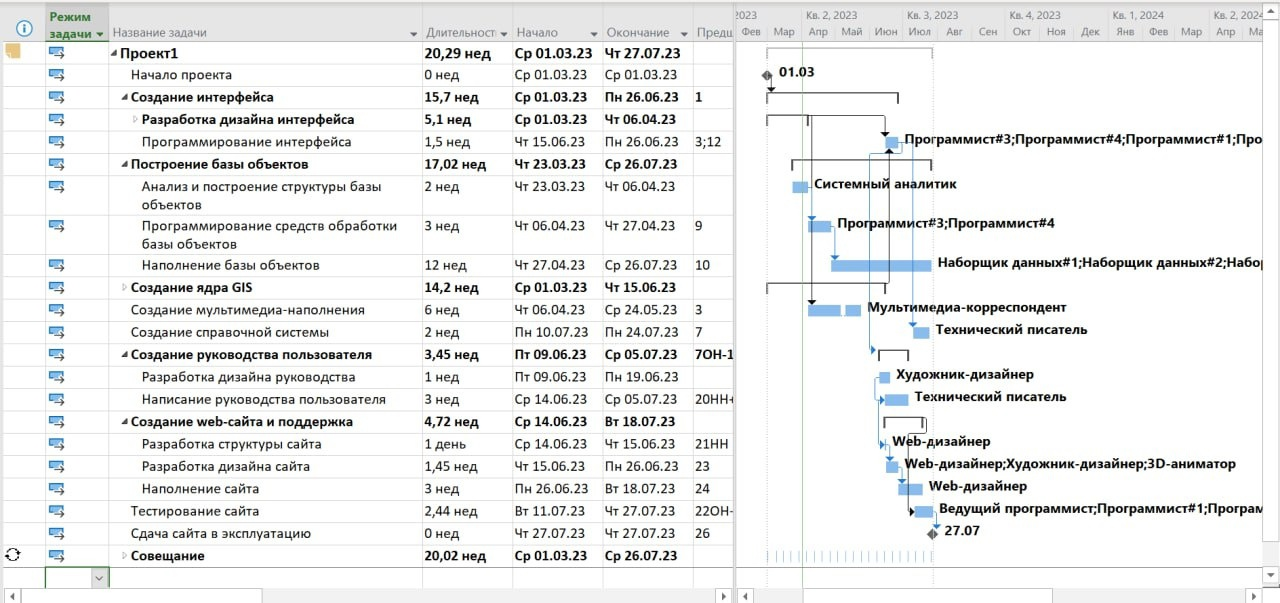
\includegraphics[scale=0.3]{inc/img/start-project.jpg}
	\end{center}
	\captionsetup{justification=centering}
	\caption{Состояние проекта}
	\label{img:start-project}
\end{figure}

Из статистики проекта, представленной на рисунке \ref{img:start-stat}, видно, что базовые затраты на проект составили 48 824.57 рублей, а трудозатраты --- 9 523 часа.

\begin{figure}[H]
	\begin{center}
		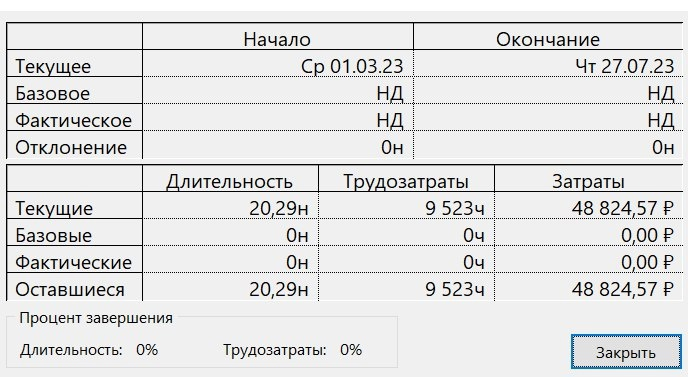
\includegraphics[scale=0.3]{inc/img/start-stat.jpg}
	\end{center}
	\captionsetup{justification=centering}
	\caption{Статистика проекта}
	\label{img:start-stat}
\end{figure}

Сведения об используемых в проекте ресурсах приведены на рисунках \ref{img:start-costs} и \ref{img:start-lcosts}.

\begin{figure}[H]
	\begin{center}
		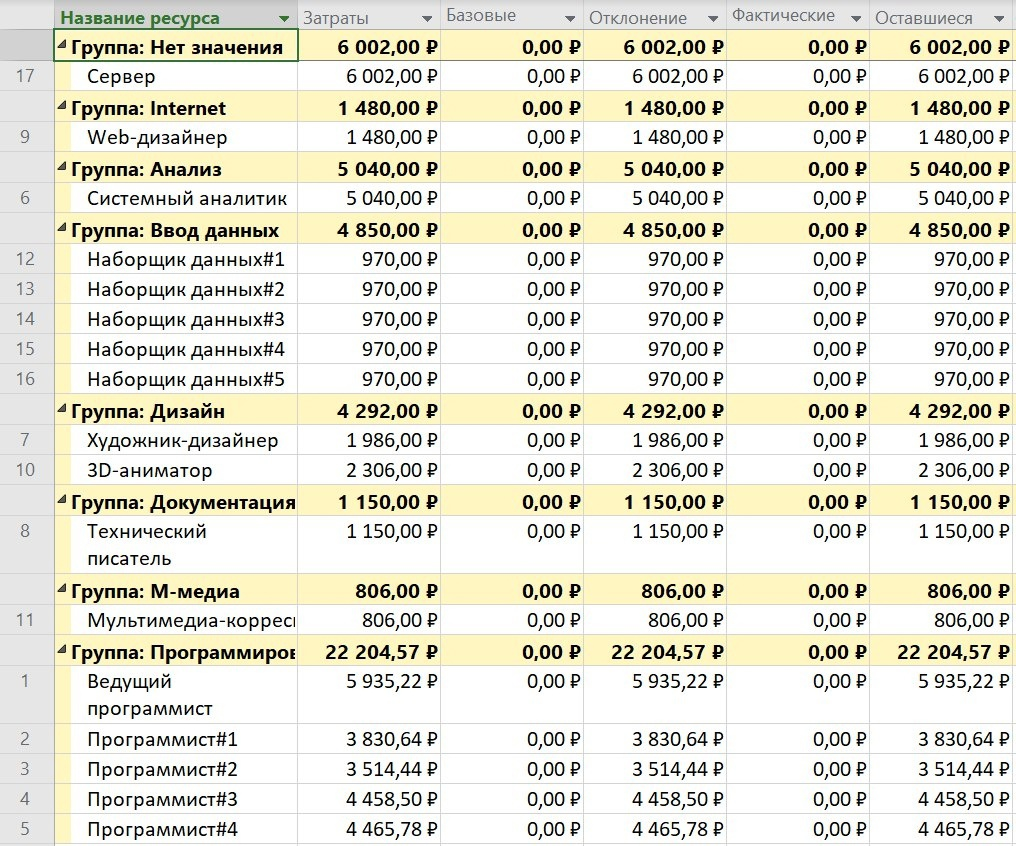
\includegraphics[scale=0.3]{inc/img/start-costs.jpg}
	\end{center}
	\captionsetup{justification=centering}
	\caption{Затраты на ресурсы}
	\label{img:start-costs}
\end{figure}

\begin{figure}[H]
	\begin{center}
		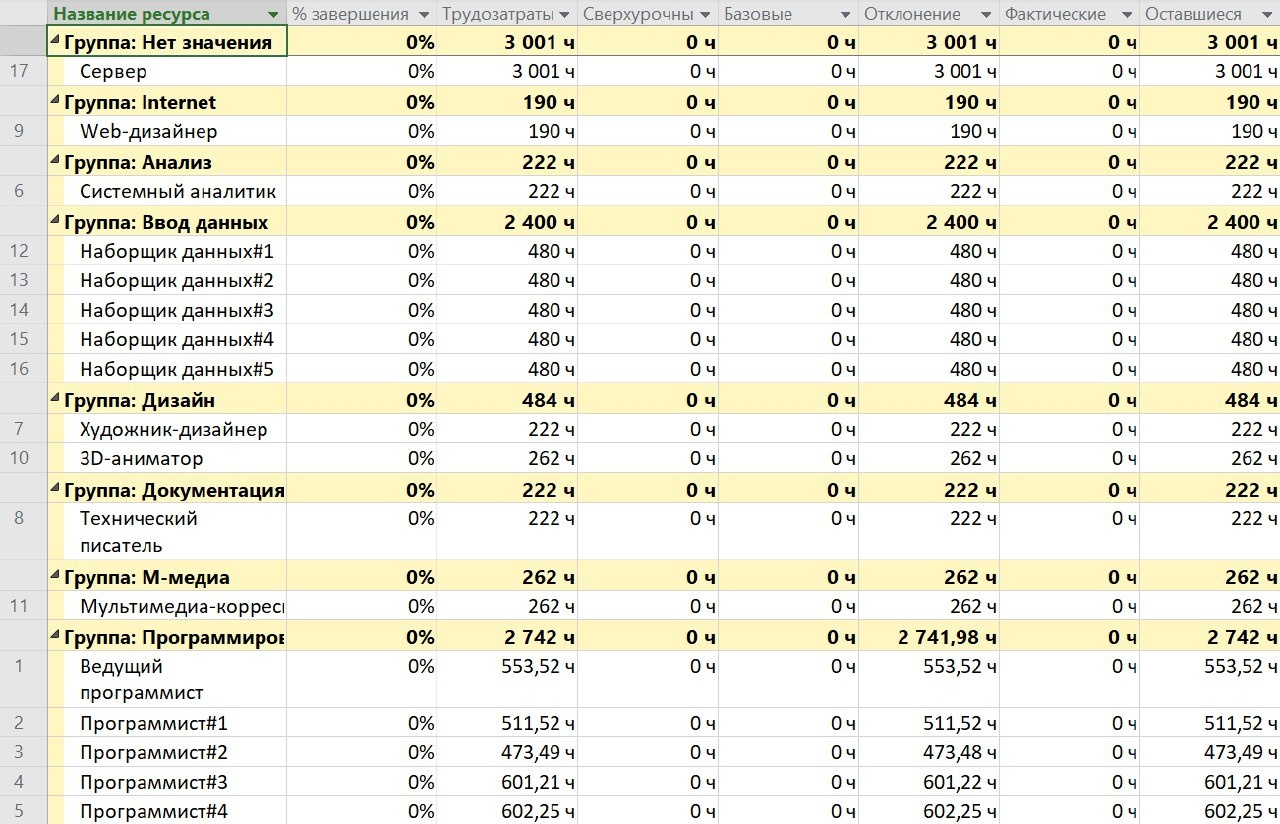
\includegraphics[scale=0.3]{inc/img/start-lcosts.jpg}
	\end{center}
	\captionsetup{justification=centering}
	\caption{Трудозатраты ресурсов}
	\label{img:start-lcosts}
\end{figure}

Ввод фактических данных о проекте осуществлялся по состоянию на 23.05.2023, установка данной даты отчета показана на рисунке \ref{img:setup-data}.

\begin{figure}[H]
	\begin{center}
		
\includegraphics[scale=0.5]{inc/img/setup-data.jpg}
	\end{center}
	\captionsetup{justification=centering}
	\caption{Установка даты отчета}
	\label{img:setup-data}
\end{figure}

\section*{Задание 1}

Задача <<Создание заставки>> закончилась на 5 дней позже. Было выполнено обновление задачи: фактическая дата окончания задачи сместилась с 6.06.2023 на 11.06.2023, как представлено на рисунке \ref{img:task1}.

\begin{figure}[H]
	\begin{center}
		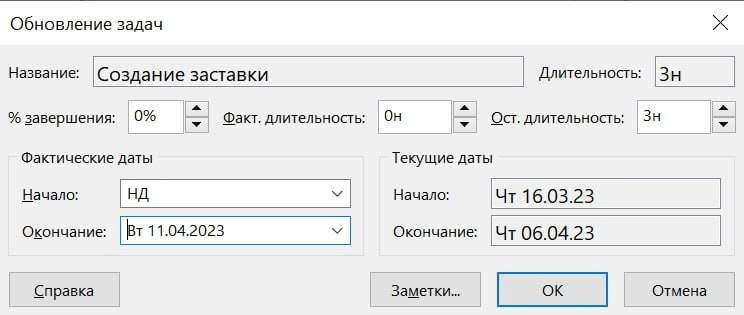
\includegraphics[scale=0.3]{inc/img/task1.jpg}
	\end{center}
	\captionsetup{justification=centering}
	\caption{Обновление задачи <<Создание заставки>>}
	\label{img:task1}
\end{figure}

Результат обновления приведен на рисунке \ref{img:task1-result}. Обновление задачи повлияло на длительность всей задачи <<Разработка дизайна интерфейса>>, после которой начинается задача <<Создание мультимедиа-наполнения>>, сроки реализации которой сдвинулись. Данная задача заканчивается раньше критических, поэтому длительность проекта не изменилась.

\begin{figure}[H]
	\begin{center}
		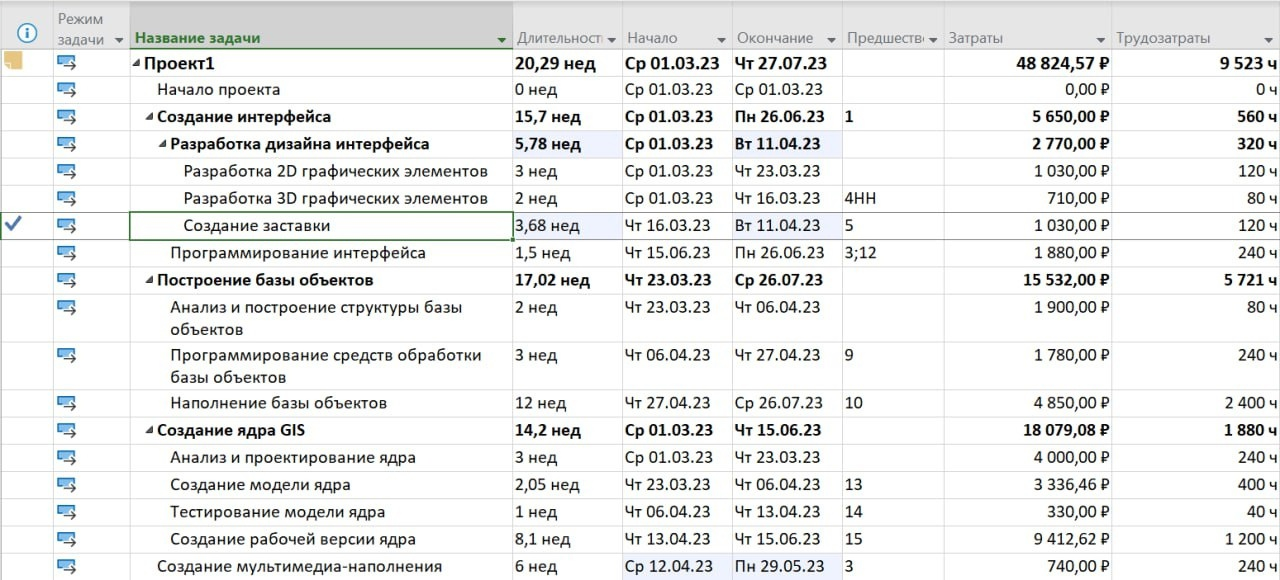
\includegraphics[scale=0.25]{inc/img/task1-result.jpg}
	\end{center}
	\captionsetup{justification=centering}
	\caption{Результат обновления задачи <<Создание заставки>>}
	\label{img:task1-result}
\end{figure}

\section*{Задание 2}

Задача <<Программирование средств обработки базы объектов>> закончилась на 7 дней раньше. Состояние задачи до обновления показано на рисунке~\ref{img:task2-before}.

\begin{figure}[H]
	\begin{center}
		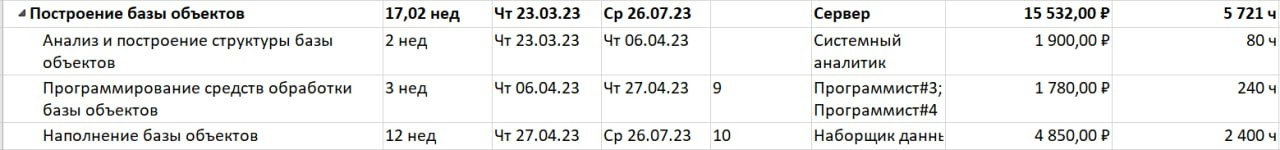
\includegraphics[scale=0.3]{inc/img/task2-before.jpg}
	\end{center}
	\captionsetup{justification=centering}
	\caption{Состояние задачи <<Программирование средств обработки базы объектов>> до обновления}
	\label{img:task2-before}
\end{figure}

Было выполнено обновление задачи: фактическая дата окончания задачи сместилась с 27.04.2023 на 20.04.2023, как представлено на рисунке \ref{img:task2}.

\begin{figure}[H]
	\begin{center}
		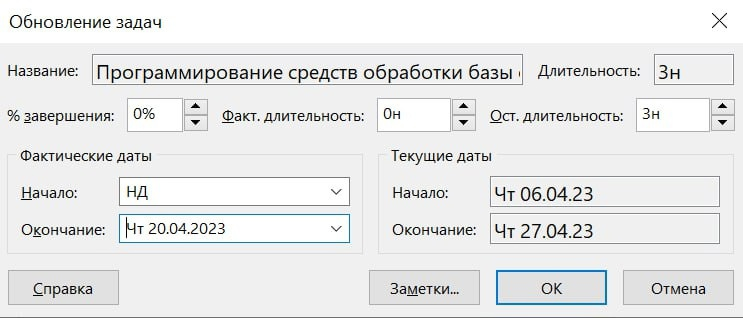
\includegraphics[scale=0.3]{inc/img/task2.jpg}
	\end{center}
	\captionsetup{justification=centering}
	\caption{Обновление задачи <<Программирование средств обработки базы объектов>>}
	\label{img:task2}
\end{figure}

Результат обновления приведен на рисунке \ref{img:task2-result}. Обновление задачи повлияло на длительность всей задачи <<Построение базы объектов>>, от которой не зависят другие задачи, поэтому длительность проекта не изменилась. При этом сократилось время использования сервера, поэтому сократились затраты на 330 рублей.

\begin{figure}[H]
	\begin{center}
		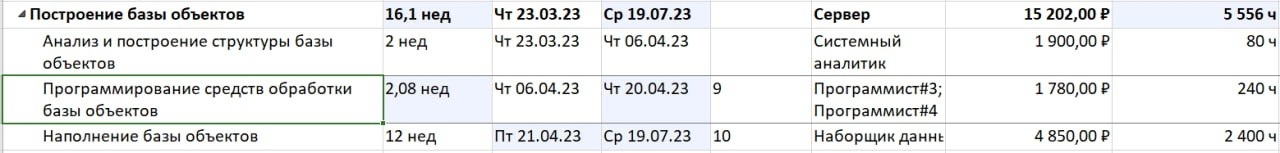
\includegraphics[scale=0.3]{inc/img/task2-result.jpg}
	\end{center}
	\captionsetup{justification=centering}
	\caption{Результат обновления задачи <<Программирование средств обработки базы объектов>>}
	\label{img:task2-result}
\end{figure}

Из-за сдвига задачи <<Программирование средств обработки базы объектов>> возникли перегрузки ресурсов <<Программист 3>> и <<Программист 4>> в связи с наложением ее сроков выполнения и сроков реализации задачи <<Создание модели ядра>>, что показано на рисунке \ref{img:task2-overloads}.

\begin{figure}[H]
	\begin{center}
		
\includegraphics[scale=0.3]{inc/img/task2-overloads.jpg}
	\end{center}
	\captionsetup{justification=centering}
	\caption{Возникшие перегрузки}
	\label{img:task2-overloads}
\end{figure}

Для их устранения были установлены задержки ресурсам <<Программист 3>> и <<Программист 4>> в один день для задачи <<Программирование средств обработки базы объектов>>, как представлено на рисунках \ref{img:task2-overloads-fix1} и \ref{img:task2-overloads-fix2}.

\begin{figure}[H]
	\begin{center}
		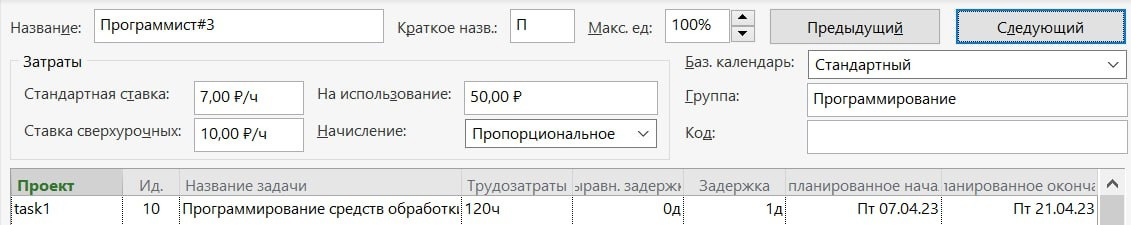
\includegraphics[scale=0.3]{inc/img/task2-fix-overloads1.jpg}
	\end{center}
	\captionsetup{justification=centering}
	\caption{Установка задержки ресурсу <<Программист 3>>}
	\label{img:task2-overloads-fix1}
\end{figure}

\begin{figure}[H]
	\begin{center}
		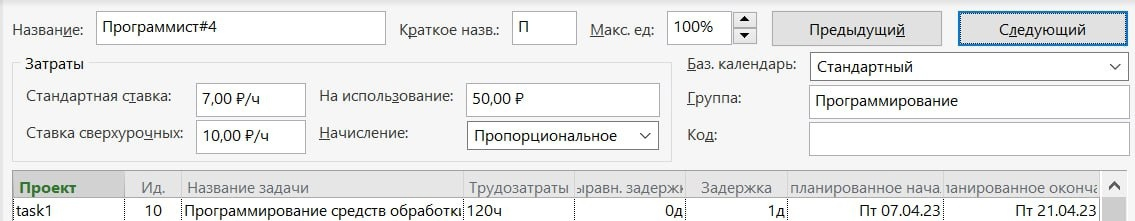
\includegraphics[scale=0.3]{inc/img/task2-fix-overloads2.jpg}
	\end{center}
	\captionsetup{justification=centering}
	\caption{Установка задержки ресурсу <<Программист 4>>}
	\label{img:task2-overloads-fix2}
\end{figure}

Результат устранения перегрузок приведен на рисунке \ref{img:task2-no-overloads}.

\begin{figure}[H]
	\begin{center}
		
\includegraphics[scale=0.3]{inc/img/task2-no-overloads.jpg}
	\end{center}
	\captionsetup{justification=centering}
	\caption{Результат устранения перегрузок}
	\label{img:task2-no-overloads}
\end{figure}

В связи с задержкой задачи затраты составили 15 250 рублей, что показано на рисунке \ref{img:task2-final}.

\begin{figure}[H]
	\begin{center}
		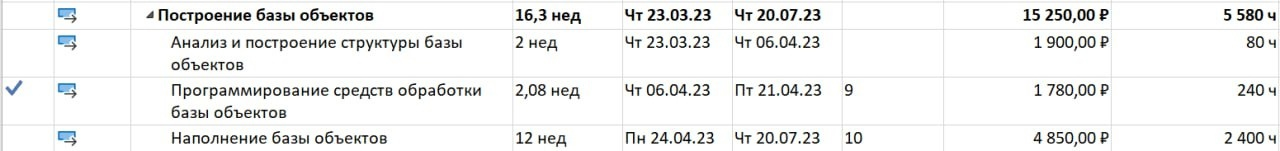
\includegraphics[scale=0.3]{inc/img/task2-final.jpg}
	\end{center}
	\captionsetup{justification=centering}
	\caption{Состояние задачи <<Построение базы объектов>>}
	\label{img:task2-final}
\end{figure}

Из текущей статистики проекта, представленной на рисунке \ref{img:task2-stat}, видно, что текущие затраты на проект составили 48 542.57 рублей, а трудозатраты --- 9 382 часа.

\begin{figure}[H]
	\begin{center}
		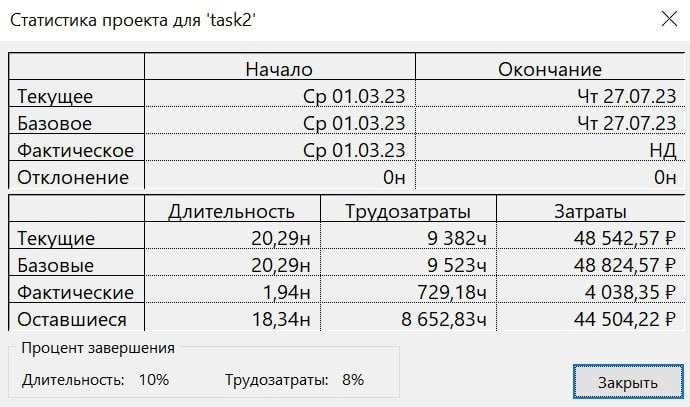
\includegraphics[scale=0.3]{inc/img/task2-stat.jpg}
	\end{center}
	\captionsetup{justification=centering}
	\caption{Текущая статистика проекта}
	\label{img:task2-stat}
\end{figure}
 
\section*{Задание 3}

Задача <<Создание мультимедиа-наполнения>> выполнена на 75\%. Было выполнено обновление задачи: процент завершения стал равным 75\%, как представлено на рисунке \ref{img:task3}.

\begin{figure}[H]
	\begin{center}
		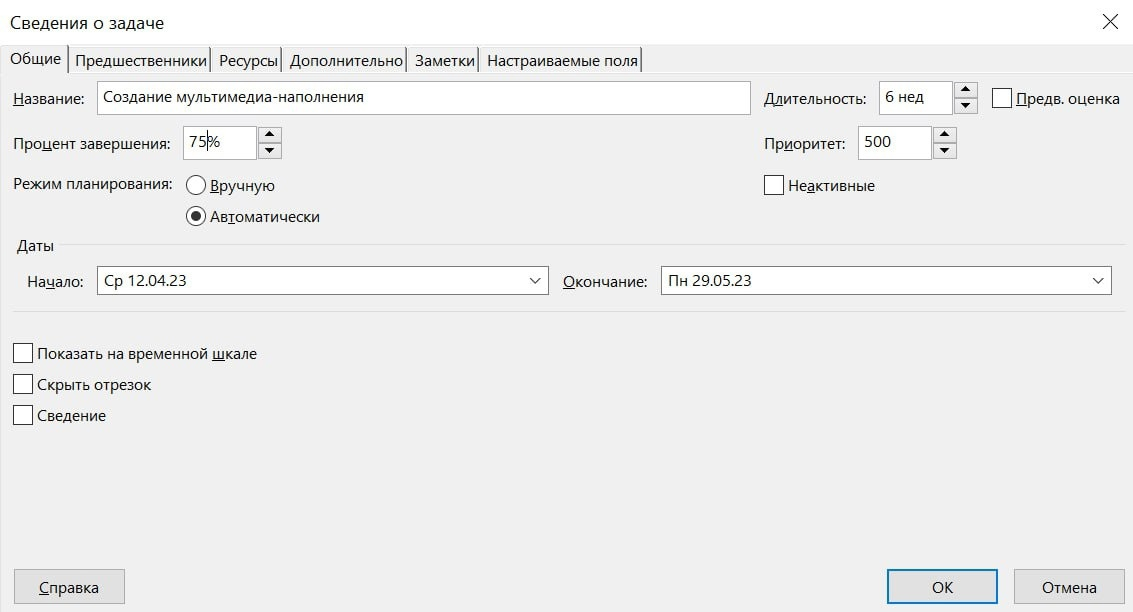
\includegraphics[scale=0.3]{inc/img/task3.jpg}
	\end{center}
	\captionsetup{justification=centering}
	\caption{Обновление задачи <<Создание мультимедиа-наполнения>>}
	\label{img:task3}
\end{figure}

Результат обновления приведен на рисунке \ref{img:task3-result}.

\begin{figure}[H]
	\begin{center}
		
\includegraphics[scale=0.3]{inc/img/task3-result.jpg}
	\end{center}
	\captionsetup{justification=centering}
	\caption{Результат обновления задачи <<Создание мультимедиа-наполнения>>}
	\label{img:task3-result}
\end{figure}

\section*{Задание 4}

24.03.2023 уволили ведущего программиста. Для учета этого обновления была изменена доступность ресурса <<Ведущий программист>>: ресурс доступен по 24.03.2023, как показано на рисунке \ref{img:task4}.

\begin{figure}[H]
	\begin{center}
		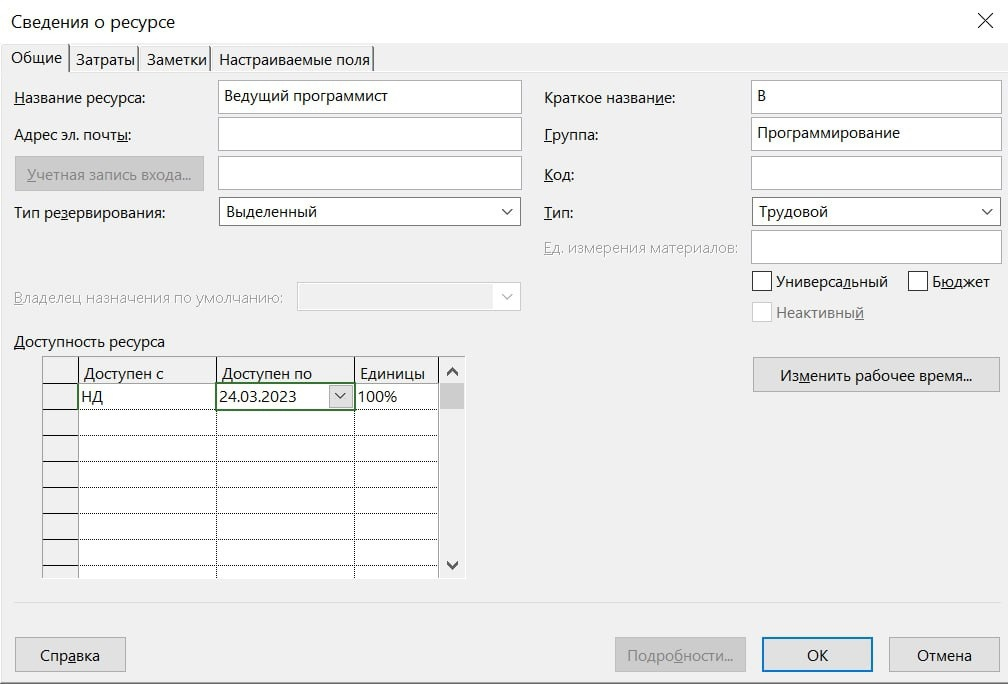
\includegraphics[scale=0.3]{inc/img/task4.jpg}
	\end{center}
	\captionsetup{justification=centering}
	\caption{Изменение доступности ресурса <<Ведущий программист>>}
	\label{img:task4}
\end{figure}

Также ресурс был удален с задач, на которые он был назначен после даты увольнения: <<Создание модели ядра>>, <<Создание рабочей версии ядра>>, <<Тестирование сайта>> и совещаний 5-22.

В результате изменений возникли перегрузки, представленные на рисунке \ref{img:task4-overloads}. Перегрузки связаны с тем, что при удалении задач сохранялся объем трудозатрат ресурсов, но увеличивалась длительность задач, и получилось наложение сроков выполнения задач <<Создание модели ядра>> и <<Программирование средств обработки базы объектов>>.

\begin{figure}[H]
	\begin{center}
		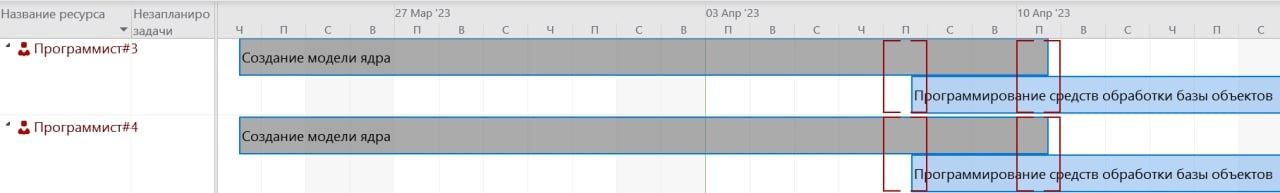
\includegraphics[scale=0.3]{inc/img/task4-overloads.jpg}
	\end{center}
	\captionsetup{justification=centering}
	\caption{Возникшие перегрузки}
	\label{img:task4-overloads}
\end{figure}

Для их устранения задержки ресурсам <<Программист 3>> и <<Программист 4>> для задачи <<Программирование средств обработки базы объектов>> были увеличены до трех дней, что приведено на рисунке \ref{img:task4-overloads-fix}.

\begin{figure}[H]
	\begin{center}
		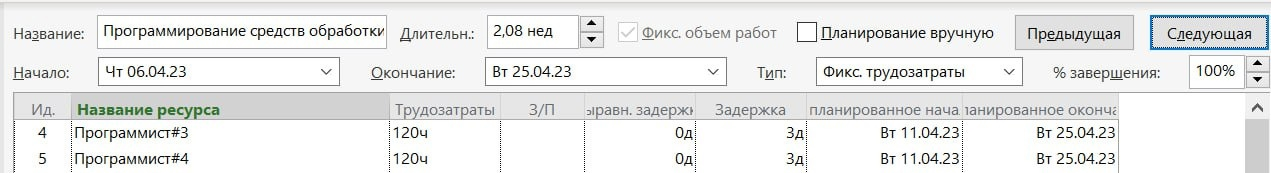
\includegraphics[scale=0.3]{inc/img/task4-fix-overloads.jpg}
	\end{center}
	\captionsetup{justification=centering}
	\caption{Установка задержек ресурсам}
	\label{img:task4-overloads-fix}
\end{figure}

Из текущей статистики проекта, показанной на рисунке \ref{img:task4-stat}, видно, что текущие затраты на проект сократились до 47 020.01 рублей, а трудозатраты увеличились до 9 460 часов.

\begin{figure}[H]
	\begin{center}
		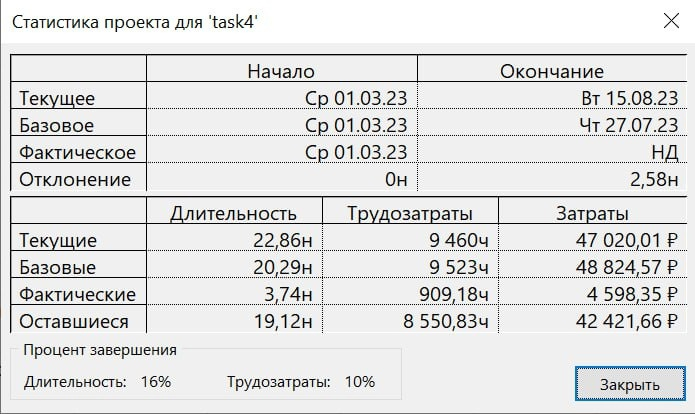
\includegraphics[scale=0.3]{inc/img/task4-stat.jpg}
	\end{center}
	\captionsetup{justification=centering}
	\caption{Текущая статистика проекта}
	\label{img:task4-stat}
\end{figure}

\section*{Задание 5}

C 1.04.2023 подняли заработную плату программистам 1-4 на 20\%. Для учета этого обновления была изменена ставка ресурсов <<Программист 1>>-<<Программист 4>>. Пример изменения ставки представлен на рисунке \ref{img:task5}.

\begin{figure}[H]
	\begin{center}
		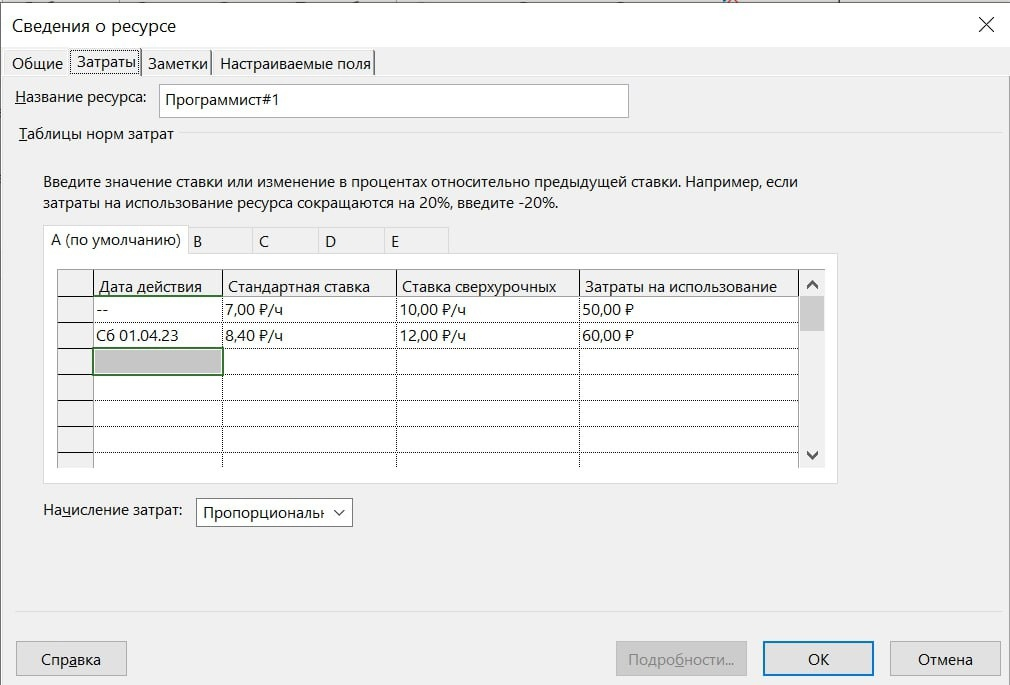
\includegraphics[scale=0.3]{inc/img/task5.jpg}
	\end{center}
	\captionsetup{justification=centering}
	\caption{Изменение ставки ресурса <<Программист 1>>}
	\label{img:task5}
\end{figure}

Из текущей статистики проекта, приведенной на рисунке \ref{img:task5-stat}, видно, что текущие затраты на проект увеличились до 50 513.21 рублей.

\begin{figure}[H]
	\begin{center}
		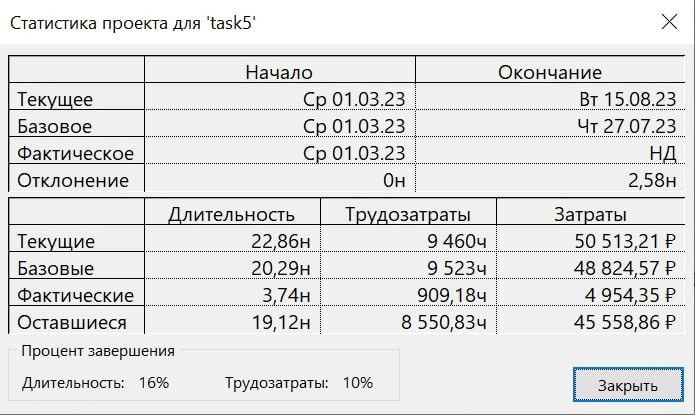
\includegraphics[scale=0.3]{inc/img/task5-stat.jpg}
	\end{center}
	\captionsetup{justification=centering}
	\caption{Текущая статистика проекта}
	\label{img:task5-stat}
\end{figure}

\section*{Задание 6}

C 1.04.2023 аренда сервера подорожала на 15\%. Для учета этого обновления была изменена ставка ресурса <<Сервер>>, что показано на рисунке~\ref{img:task6}.

\begin{figure}[H]
	\begin{center}
		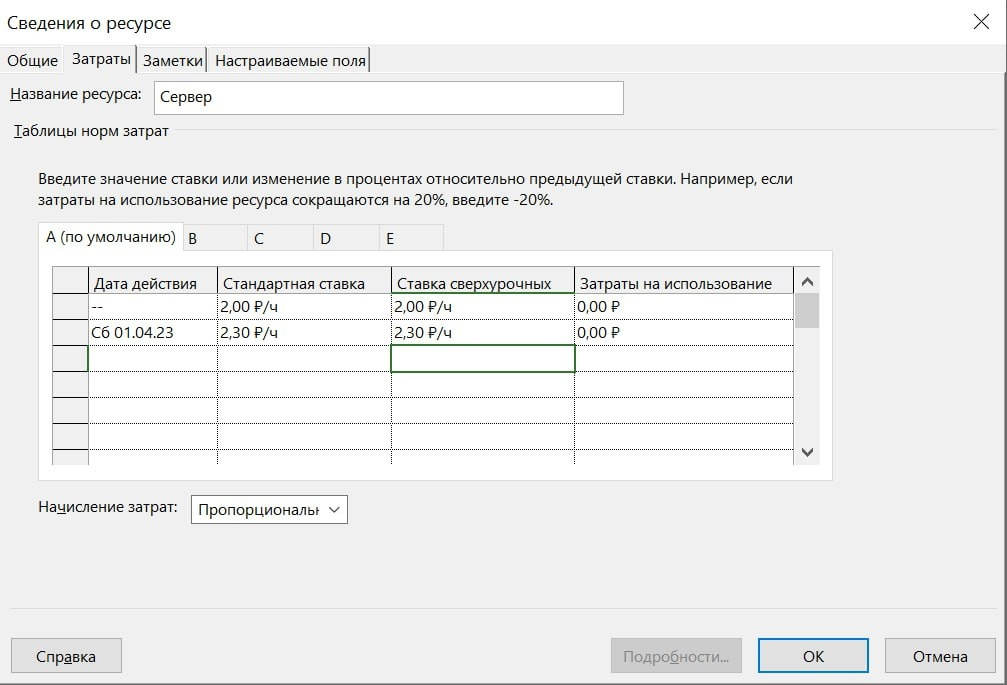
\includegraphics[scale=0.25]{inc/img/task6.jpg}
	\end{center}
	\captionsetup{justification=centering}
	\caption{Изменение ставки ресурса <<Сервер>>}
	\label{img:task6}
\end{figure}

Из текущей статистики проекта, предствленной на рисунке \ref{img:task6-stat}, видно, что текущие затраты на проект увеличились до 51 336.71 рублей.

\begin{figure}[H]
	\begin{center}
		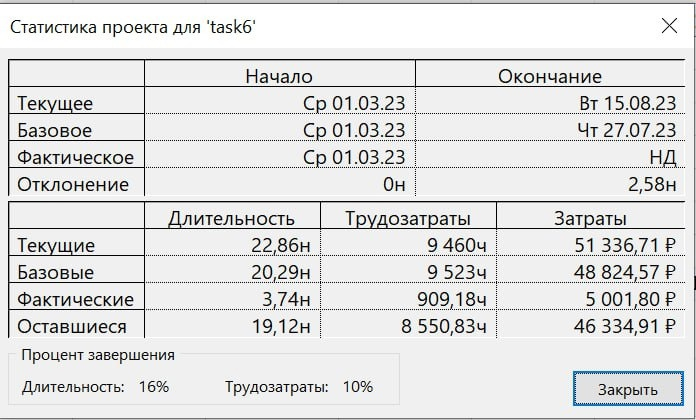
\includegraphics[scale=0.3]{inc/img/task6-stat.jpg}
	\end{center}
	\captionsetup{justification=centering}
	\caption{Текущая статистика проекта}
	\label{img:task6-stat}
\end{figure}

\section*{Задание 7}

C 1.04.2023 начали проводиться презентации раз в две недели по часу, для каждого из которых нужна пачка бумаги стоимостью 100 рублей. Для учета этого обновления была создана повторяющая задача <<Презентация>>, как приведено на рисунке~\ref{img:task7}.

\begin{figure}[H]
	\begin{center}
		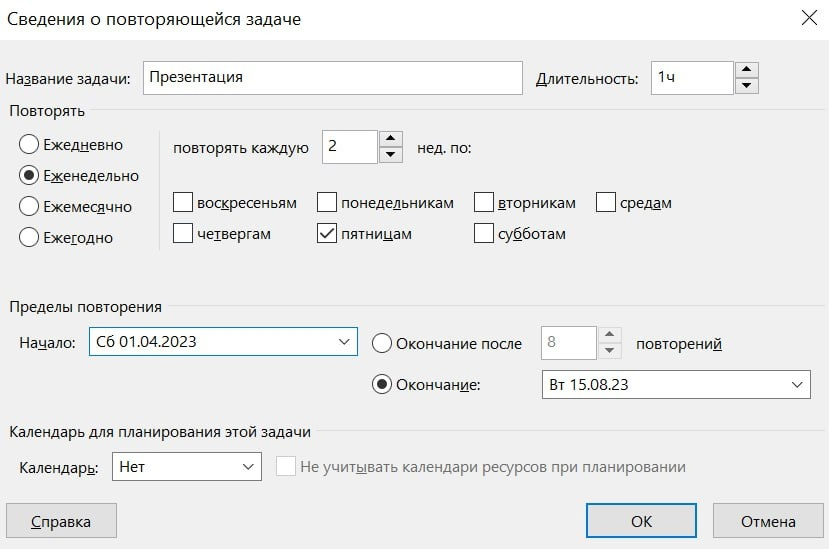
\includegraphics[scale=0.25]{inc/img/task7.jpg}
	\end{center}
	\captionsetup{justification=centering}
	\caption{Создание повторяющейся задачи <<Презентация>>}
	\label{img:task7}
\end{figure}

Был создан материальный ресурс <<Бумага>> со стандартной ставкой 100 рублей, как показано на рисунке \ref{img:task7-paper}. Ресурс был назначен повторяющейся задаче, что представлено на рисунке \ref{img:task7-alignment}.

\begin{figure}[H]
	\begin{center}
		
\includegraphics[scale=0.25]{inc/img/task7-paper.jpg}
	\end{center}
	\captionsetup{justification=centering}
	\caption{Создание материального ресурса <<Бумага>>}
	\label{img:task7-paper}
\end{figure}

\begin{figure}[H]
	\begin{center}
		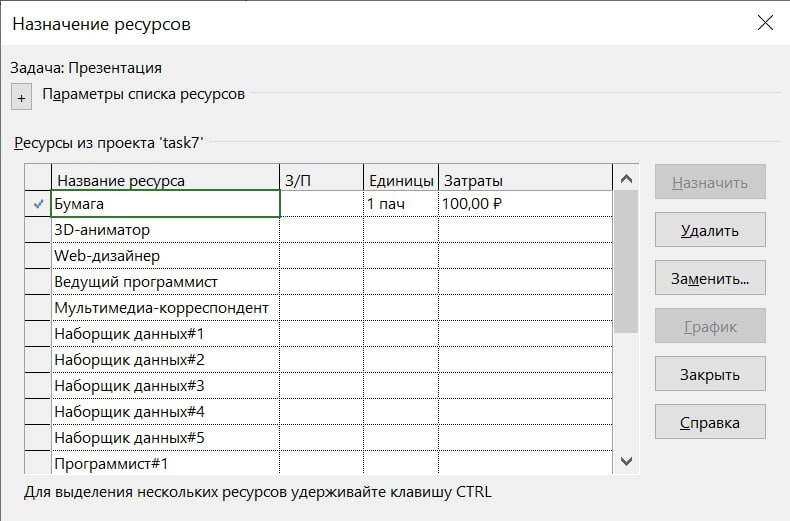
\includegraphics[scale=0.25]{inc/img/task7-alignment-paper.jpg}
	\end{center}
	\captionsetup{justification=centering}
	\caption{Назначение ресурса повторяющейся задаче}
	\label{img:task7-alignment}
\end{figure}

Результат добавления фактических данных приведен на рисунке \ref{img:task7-result}.

\begin{figure}[H]
	\begin{center}
		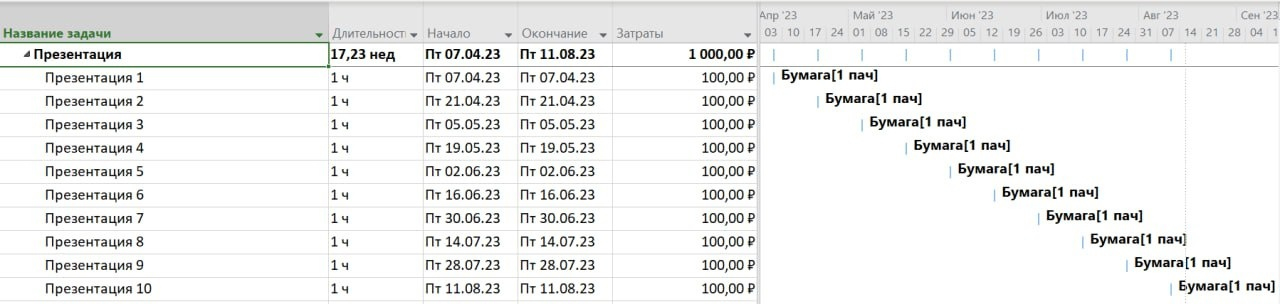
\includegraphics[scale=0.25]{inc/img/task7-result.jpg}
	\end{center}
	\captionsetup{justification=centering}
	\caption{Результат добавления повторяющейся задачи <<Презентация>>}
	\label{img:task7-result}
\end{figure}

Из текущей статистики проекта, показанной на рисунке \ref{img:task7-stat}, видно, что текущие затраты на проект увеличились до 52 336.71 рублей.

\begin{figure}[H]
	\begin{center}
		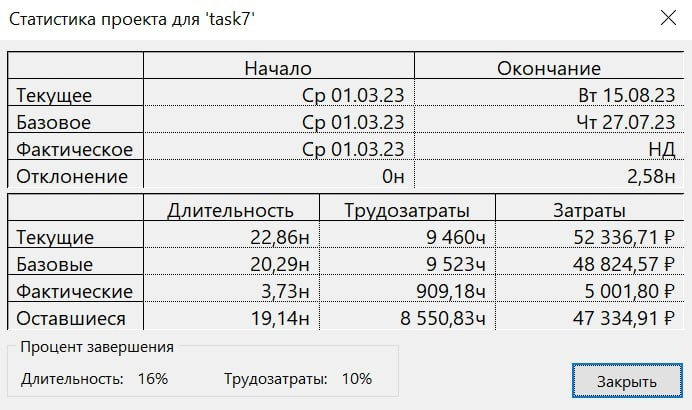
\includegraphics[scale=0.3]{inc/img/task7-stat.jpg}
	\end{center}
	\captionsetup{justification=centering}
	\caption{Текущая статистика проекта}
	\label{img:task7-stat}
\end{figure}

\section*{Задание 8}

C 1.04.2023 в еженедельных совещаниях стали принимать участие только те сотрудники, у которых есть задачи на текущей неделе. Для учета этого обновления у задач были удалены ресурсы, которые не должны присутствовать на совещании в соответствии со своими задачами. Пример изменения представлен на рисунке~\ref{img:task8}.

\begin{figure}[H]
	\begin{center}
		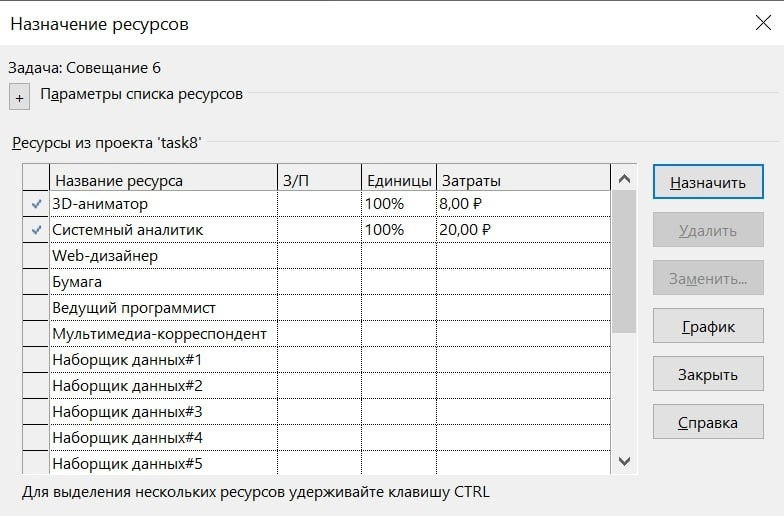
\includegraphics[scale=0.25]{inc/img/task8.jpg}
	\end{center}
	\captionsetup{justification=centering}
	\caption{Обновление ресурсов для совещания 6}
	\label{img:task8}
\end{figure}

Результат изменения ресурсов, участвующих в совещаниях, приведен на рисунке \ref{img:task8-result}.

\begin{figure}[H]
	\begin{center}
		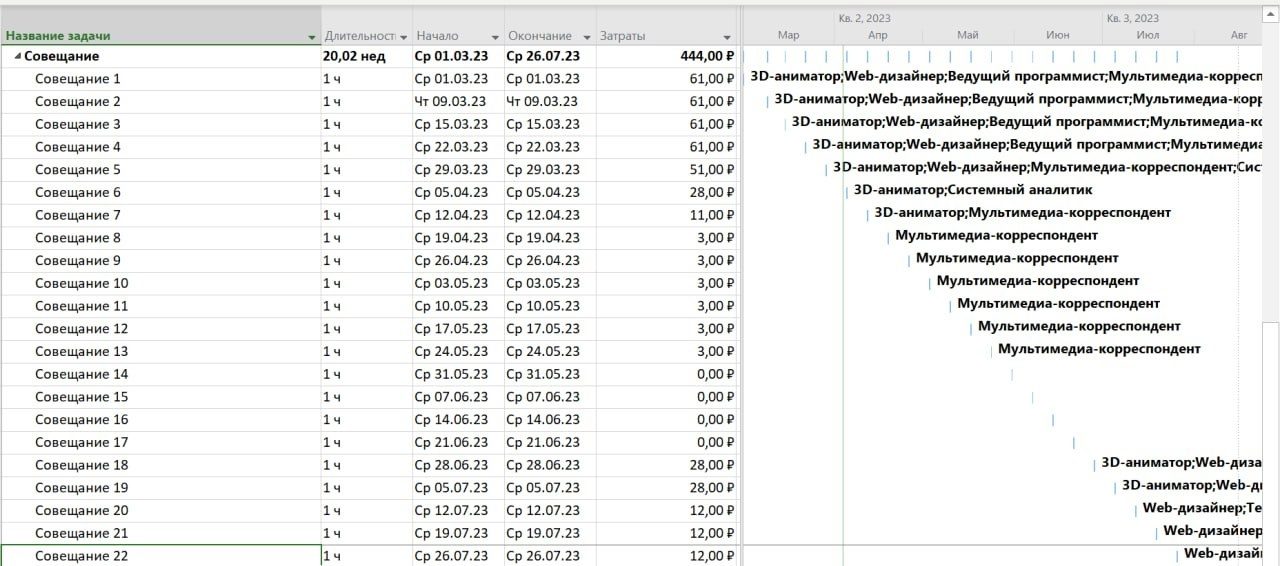
\includegraphics[scale=0.25]{inc/img/task8-result.jpg}
	\end{center}
	\captionsetup{justification=centering}
	\caption{Результат изменения ресурсов, участвующих в совещаниях}
	\label{img:task8-result}
\end{figure}

Из текущей статистики проекта, показанной на рисунке \ref{img:task8-stat}, видно, что текущие затраты на проект сократились до 51 618.71 рублей, а трудозатраты --- до 9 382 часов.

\begin{figure}[H]
	\begin{center}
		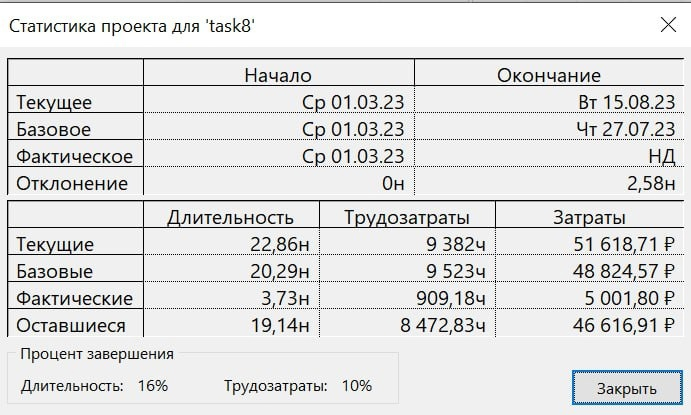
\includegraphics[scale=0.3]{inc/img/task8-stat.jpg}
	\end{center}
	\captionsetup{justification=centering}
	\caption{Текущая статистика проекта}
	\label{img:task8-stat}
\end{figure}

\section*{Анализ актуализированного состояния проекта}

На основе базового плана была выведена текущая линия прогресса (рисунок \ref{img:analysis}), представленная на рисунке \ref{img:progress-line}.

\begin{figure}[H]
	\begin{center}
		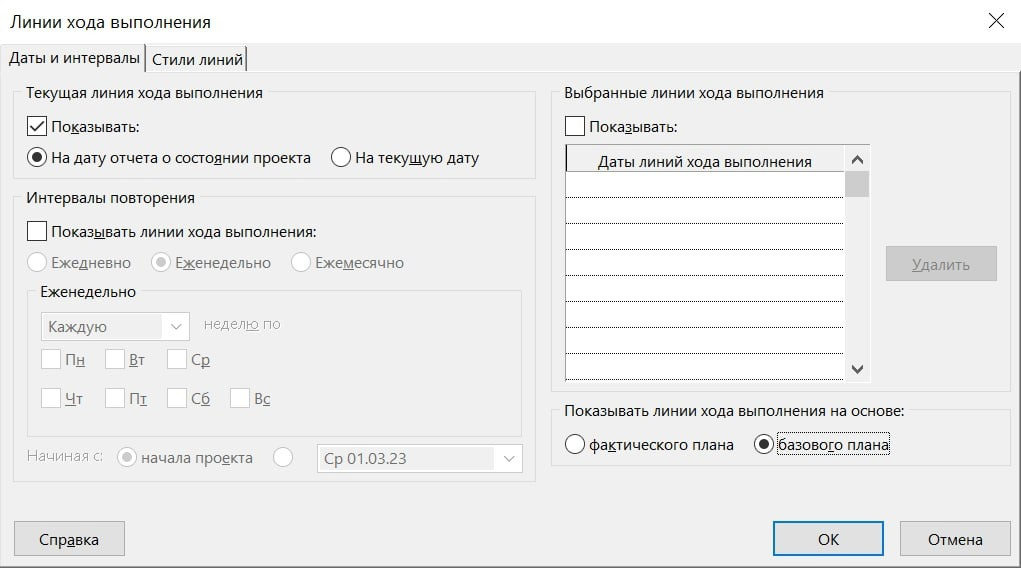
\includegraphics[scale=0.25]{inc/img/analysis.jpg}
	\end{center}
	\captionsetup{justification=centering}
	\caption{Вывод текущей линии прогресса}
	\label{img:analysis}
\end{figure}

\begin{figure}[H]
	\begin{center}
		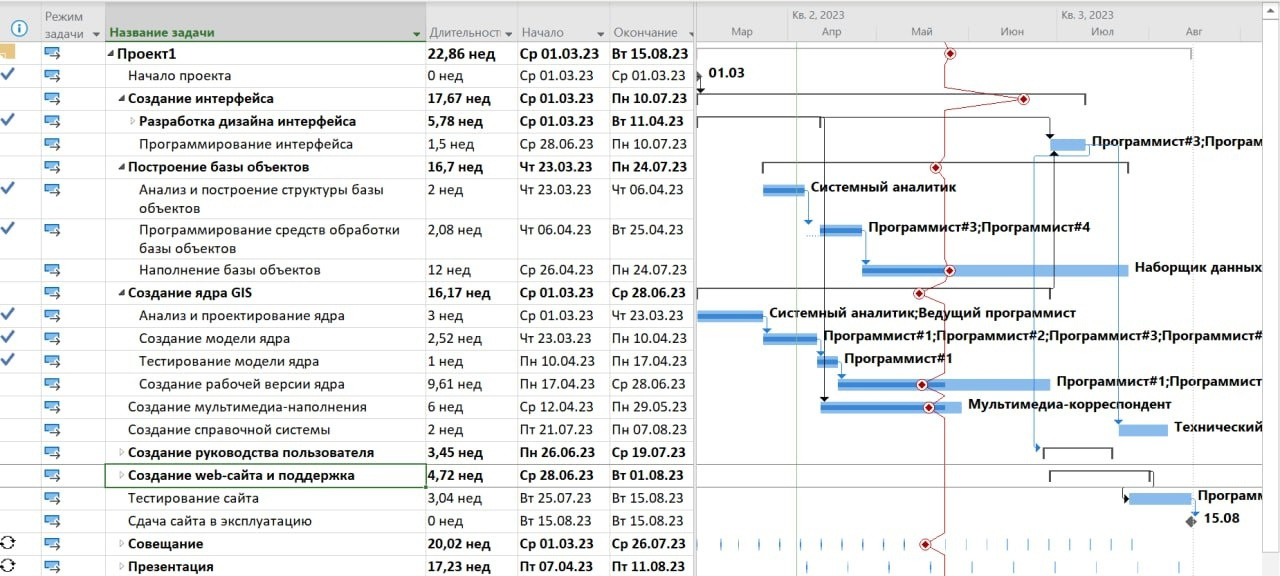
\includegraphics[scale=0.3]{inc/img/progress-line.jpg}
	\end{center}
	\captionsetup{justification=centering}
	\caption{Текущая линия прогресса}
	\label{img:progress-line}
\end{figure}

Плановые и фактические показатели проекта и отклонения представлены на рисунке \ref{img:deviation}.

\begin{figure}[H]
	\begin{center}
		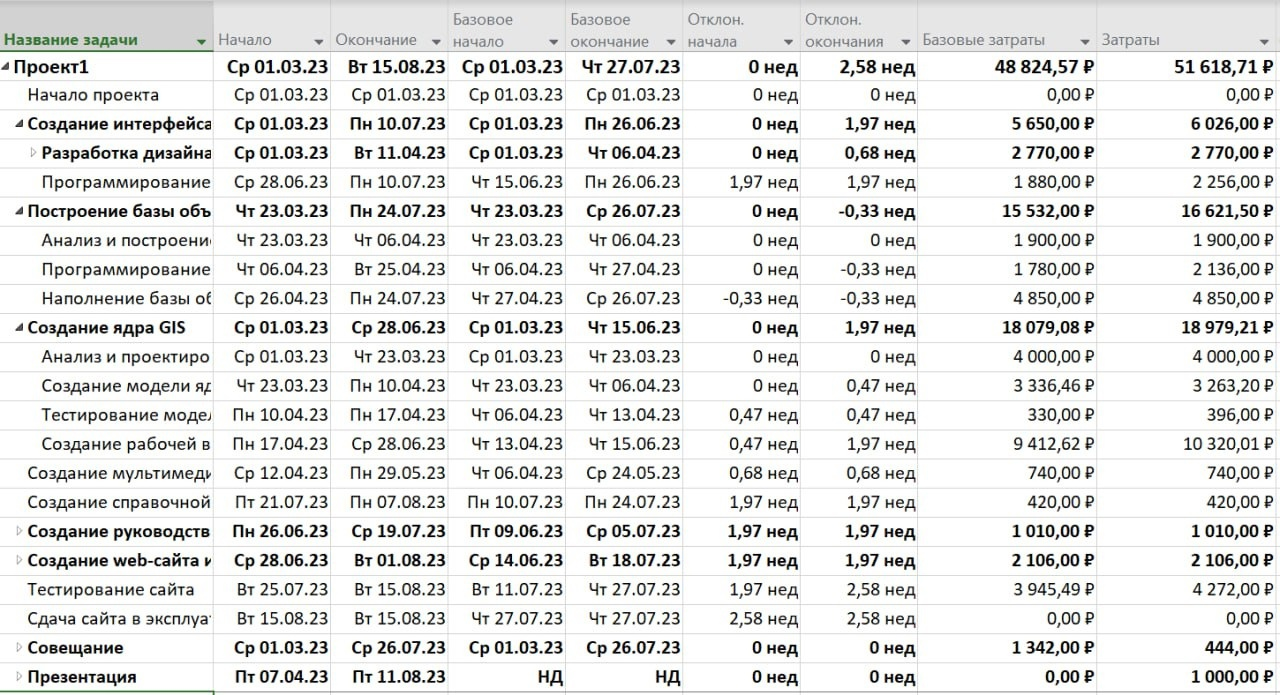
\includegraphics[scale=0.3]{inc/img/deviation.jpg}
	\end{center}
	\captionsetup{justification=centering}
	\caption{Отклонения от базового плана}
	\label{img:deviation}
\end{figure}

В результате их сравнения можно сделать вывод о том, что затраты на проект увеличились с 48 824.57 рублей до 51 618.71 рублей (разница в 2 794.14 рублей), дата окончания сдвинулась с 27.07.2023 на 15.08.2023, длительность увеличилась на 19 дней.

Длительность проекта удовлетворяет заявленному сроку, но затраты проекта не умещаются в бюджет. Необходима оптимизация затрат. 

\section*{Стратегия устранения отклонений затрат}

Увеличение затрат проекта связано с повышением заработной платы программистов 1-4, проведением презентаций и подорожанием аренды сервера. Для устранения отклонений затрат можно отказаться от аренды сервера и купить собственный сервер.

Купим собственный сервер за 1000 рублей (рисунки \ref{img:new-server}-\ref{img:alignment-server}) и откажемся от аренды сервера (рисунок \ref{img:delete-server}).

\begin{figure}[H]
	\begin{center}
		
\includegraphics[scale=0.3]{inc/img/new-server.jpg}
	\end{center}
	\captionsetup{justification=centering}
	\caption{Покупка собственного сервера}
	\label{img:new-server}
\end{figure}

\begin{figure}[H]
	\begin{center}
		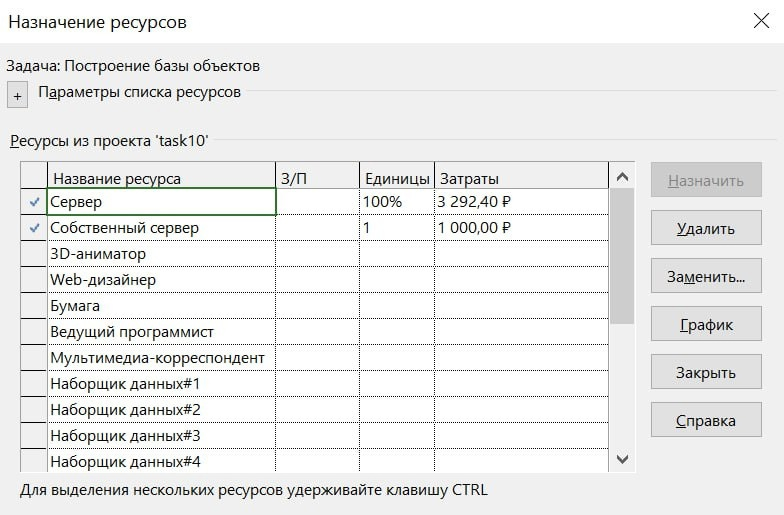
\includegraphics[scale=0.3]{inc/img/alignment-server.jpg}
	\end{center}
	\captionsetup{justification=centering}
	\caption{Назначение собственного сервера задаче}
	\label{img:alignment-server}
\end{figure}

\begin{figure}[H]
	\begin{center}
		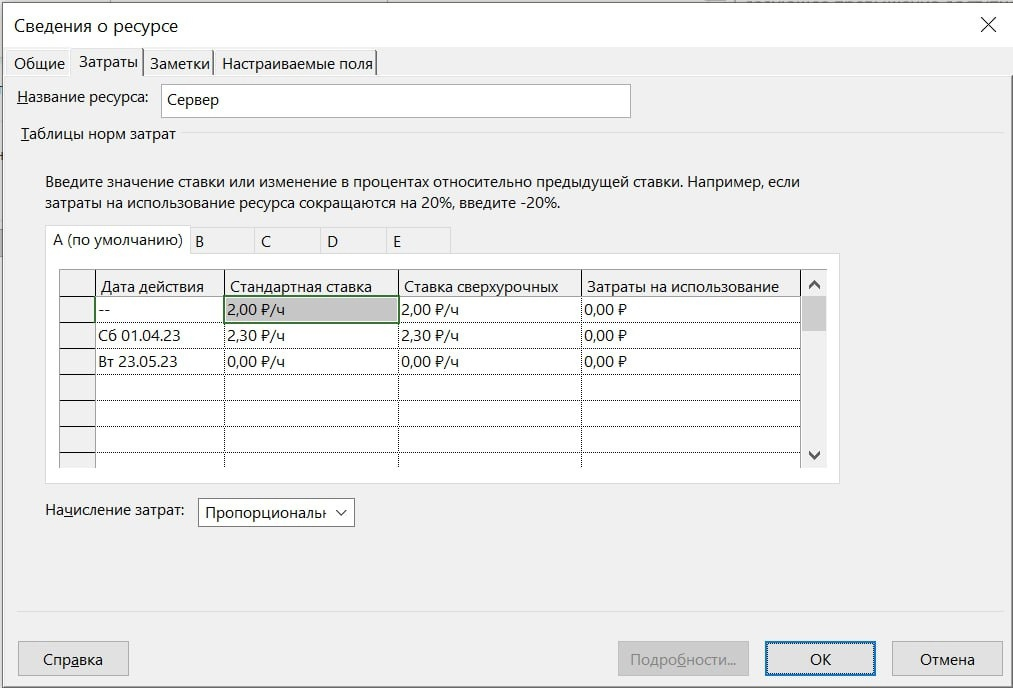
\includegraphics[scale=0.25]{inc/img/delete-server.jpg}
	\end{center}
	\captionsetup{justification=centering}
	\caption{Отказ от аренды сервера}
	\label{img:delete-server}
\end{figure}

Тогда фактические затраты на проект сократятся до 49 175.61 рублей (рисунок \ref{img:result}), что удовлетворяет установленному бюджету проекта.

\begin{figure}[H]
	\begin{center}
		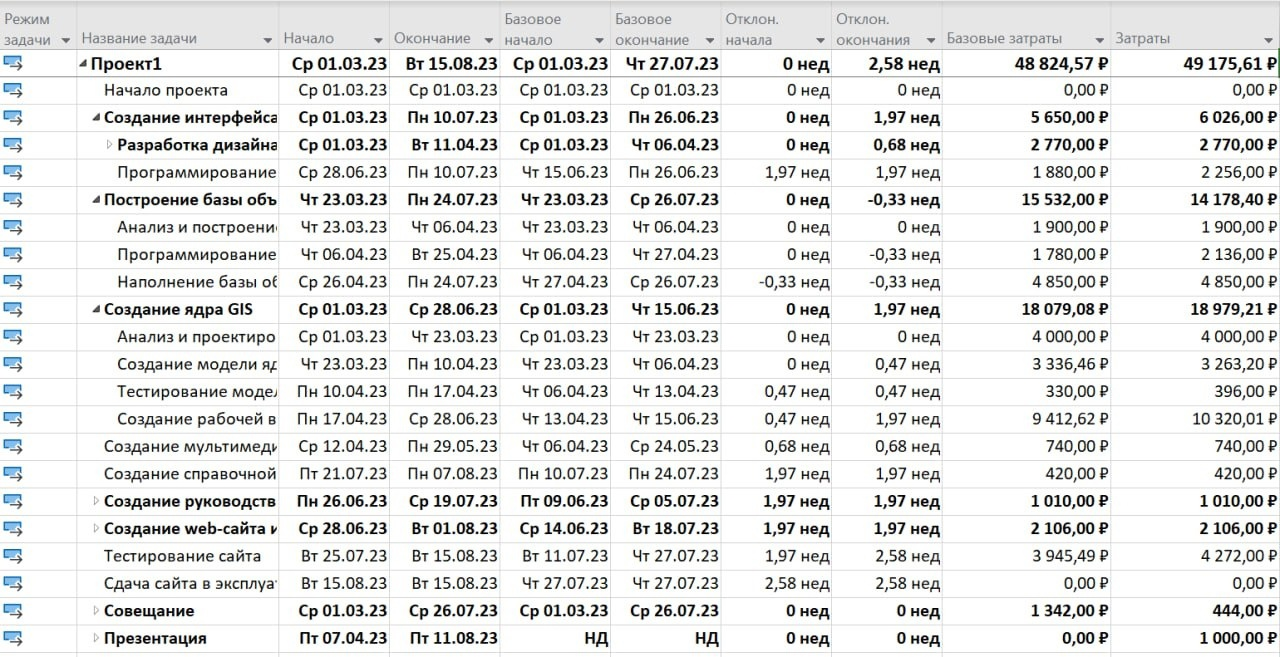
\includegraphics[scale=0.3]{inc/img/result.jpg}
	\end{center}
	\captionsetup{justification=centering}
	\caption{Отклонения от базового плана}
	\label{img:result}
\end{figure}

\section*{Вывод}

При выполнении лабораторной работы были отработаны навыки использования программы Microsoft Project для контроля за ходом реализации проекта.

После актуализации проекта его длительность увеличилась, но осталась в допустимых значениях, затраты на проект превысили установленный предел. Было предложено отказаться от аренды сервера и купить собственный, в результате чего можно сократить затраты на проект.
